\documentclass[journal]{IEEEtran}
\usepackage[T1]{fontenc}
\usepackage[utf8]{inputenc}
\usepackage{lmodern}
\usepackage{textcomp}
\usepackage{amsmath}
\usepackage{amssymb}
\usepackage{graphicx}
\usepackage{booktabs}
\usepackage{array}
\usepackage{url}
\usepackage{xcolor}

% match the manuscript's arabic section cross-references (Section 3, 5.1, ...)
\renewcommand{\thesection}{\arabic{section}}
\renewcommand{\thesubsection}{\thesection.\arabic{subsection}}
% IEEEtran prints headings via the *dis macros; override subsection display
% so it reads "5.1" (arabic) instead of the default "A."
\makeatletter
\def\thesubsectiondis{\thesection.\arabic{subsection}}
\makeatother

% pandoc helper macros (fragment mode, no template)
\providecommand{\tightlist}{\setlength{\itemsep}{0pt}\setlength{\parskip}{0pt}}
\providecommand{\passthrough}[1]{#1}

\begin{document}

\title{Protocol-Valid Faithfulness Evaluation for\\ ML-Based Network Traffic Classifiers}
\author{Nakul~Sinha%
\thanks{Manuscript prepared for the IEEE Transactions on Network and Service Management (TNSM). Citation keys resolve against \texttt{refs.bib}; figures are in \texttt{figures/}.}}

\maketitle

\begin{abstract}
Deep learning has become the default tool for network traffic
classification and intrusion detection, and with it a large literature
that attaches post-hoc explanation methods (SHAP, LIME, saliency) to
these models to make them trustworthy. That literature almost never
checks whether the explanations are \emph{correct}: in a survey of 107
works, only five define any explanation-quality metric, and none has a
dataset with ground-truth feature importance. We show that the standard
way faithfulness \emph{is} measured elsewhere, deletion/occlusion of
``important'' features, is not merely unvalidated for network traffic
but protocol-invalid: setting a feature to zero produces a packet that
violates protocol grammar (a broken checksum, an impossible length) and
does not arise from a conforming sender, so the model is queried
off-manifold. We introduce \textbf{PacketDO}, a protocol-valid
intervention operator that resamples a protocol field from its pooled
empirical marginal and recomputes every dependent field, yielding a
counterfactual that is a well-formed packet by construction. Using
PacketDO we build, to our knowledge, the first protocol-valid
interventional ground truth for traffic classifiers (necessity,
sufficiency, and a redundancy degree $R(M)$ measured by intervention, not
assumed) and audit eight widely used attribution methods (integrated
gradients, gradient saliency, DeepSHAP, occlusion, KernelSHAP, LIME,
TreeSHAP, and impurity) against it, on models with planted shortcuts of
graded strength, on flow-level real data with documented artifacts, and
on two real packet-capture corpora at the byte level. We find that
explainers reliably rank a model's true shortcut at the top yet
simultaneously attribute high importance to redundant features the model
provably does not use; that even exact Shapley values (TreeSHAP) exhibit
this false confidence when a model commits to one of several equivalent
shortcuts; and that an explainer's faithfulness ranking can flip
depending on whether features are removed by zero-masking or by
PacketDO. On real captured packets the operator gap is larger than on
synthetic traffic (zero-masking valid for 6\% of field interventions
versus 100\% for PacketDO) and the false confidence reproduces; on an
attention-based Transformer, attention weights are the least faithful
explanation of those we audit; the false confidence persists on the
pretrained ET-BERT, which we find holds three substitutable shortcuts
($R(M)$=3). We release the operator, the benchmark, and the ground-truth
tables.
\end{abstract}

\begin{IEEEkeywords}
Explainable AI, network traffic classification, feature attribution, faithfulness evaluation, counterfactual intervention, shortcut learning.
\end{IEEEkeywords}

\section{Introduction}

Machine learning now underpins a large fraction of deployed network
traffic analysis: encrypted traffic classification, application
identification, and network intrusion detection are all dominated by
deep models that operate on raw packet bytes or on flow-level feature
vectors \cite{wang2017endtoend,lotfollahi2020deeppacket,lin2022etbert}.
Because these models are opaque and because operators are reluctant to
act on decisions they cannot interrogate, a second, rapidly growing
literature attaches post-hoc explanation methods (SHAP, LIME, gradient
saliency, attention maps) to traffic classifiers, and presents the
resulting feature-importance scores as evidence that the model is
trustworthy. This explainability literature is now large enough to have
its own surveys \cite{nascita2025survey}.

What almost none of it does is check whether the explanations are
\emph{correct}. In a recent systematic survey of 107 works on
explainable AI for network traffic analysis \cite{nascita2025survey},
only five define any explanation-quality metric at all, and the survey
reports that no public traffic dataset carries ground-truth feature
importance against which an explanation could be scored. In practice,
explanations are displayed as plots and declared meaningful. The few
papers that do attempt a quantitative check substitute a proxy: either
agreement with what a human analyst expects (which measures
plausibility, not faithfulness \cite{jacovi2020towards}), or a deletion
test that removes the features an explainer called important and
measures how much the prediction changes.

This deletion test is the standard notion of faithfulness imported from
computer vision and NLP \cite{samek2017evaluating,deyoung2020eraser},
and it is the quiet foundation under most quantitative claims in the
field. Our starting observation is that it is not merely unvalidated for
network traffic: it is protocol-invalid. Removing a feature by setting
it to zero, the default in every deletion, occlusion, and AOPC-style
metric, produces a byte string that is no longer a well-formed packet:
its header checksum no longer matches its contents, or its length field
disagrees with its actual length. Such a packet is not produced by any
conforming sender, so the model is being queried outside the
distribution it was trained on, and the resulting ``importance'' is
partly an artifact of that extrapolation. (Malformed packets do occur in
practice, from NIC checksum offload or as adversarial inputs; our claim
is distributional, that zero-masked packets are absent from the
conforming traffic these classifiers are trained on, not that they can
never be observed. We return to this in Section 8.) The problem is
strictly worse than the analogous critique in vision
\cite{hooker2019benchmark,rong2022consistent}, because a packet's fields
are bound to one another by protocol grammar: you cannot change one
field and leave the rest untouched and still have a legal packet.

There is a second, deeper problem that the traffic-classification
setting makes unusually visible. Traffic datasets are riddled with
\emph{shortcuts} \cite{geirhos2020shortcut}, features that predict the
label in the dataset without reflecting any real property of the
traffic, such as the fixed time-to-live of the machine that generated a
class of attacks, or an artifact of the flow-metering tool
\cite{engelen2021troubleshooting}. A model that learns a shortcut can be
perfectly accurate on held-out data and still be wrong about the world.
The most striking published demonstration of the danger for explanations
comes from TRUSTEE \cite{jacobs2022trustee}: a decision-tree surrogate
that reproduced a traffic classifier's decisions with perfect fidelity
(an F1 of 1.00) identified three specific header bytes as the basis of
its decisions; yet when the authors tampered with exactly those three
bytes, the model's accuracy did not move, because it had learned several
mutually substitutable shortcuts and simply fell back on another. A
perfect-fidelity explanation was causally wrong. This failure mode,
redundant shortcuts that make the target of an explanation non-unique,
has never been systematically measured, in traffic classification or
anywhere else.

The two literatures that would need to meet in order to address this do
not. On one side, the explainability-for-security literature produces
attributions and never intervenes on the model to check them. On the
other, a rigour-focused strand of networking research (TRUSTEE
\cite{jacobs2022trustee}, the 2025 IEEE S\&P systematization of
encrypted-traffic classifiers \cite{wickramasinghe2025sok}, and recent
shortcut-detection frameworks
\cite{wang2026biasseeker,zhao2026shortcutcatcher}) routinely intervenes
on traffic (occluding fields, tampering bytes, ablating features) to
expose what models really use, but never calls these interventions
explanations and never evaluates an explainer with them. As a concrete
measure of the gap: the S\&P 2025 systematization runs 348 feature
occlusion experiments and contains not a single occurrence of the words
explainable, interpretable, SHAP, attribution, or saliency.

We argue that networking is, in fact, the ideal setting in which to
close this gap, for a reason that does not hold in vision or NLP:
interventional ground truth for explanations can be constructed exactly
and on-manifold. Protocol field semantics are known, so an attribution
has a defined referent; and packets are rewritable, so a field can be
set to a chosen value and the packet regenerated as a legal packet.
Ground-truth evaluation of feature attribution has been established in
vision (by pasting known objects into images \cite{yang2019bam}) and in
NLP (by injecting known lexical shortcuts into text
\cite{bastings2022shortcuts}), and in both cases it revealed that
popular attribution methods produce false-positive explanations. Neither
has ever been done for network traffic, the one modality where the
intervention that defines the ground truth is exact,
protocol-structured, and produces inputs the model could actually
receive.

This paper builds that missing instrument and uses it. Our contributions
are:

\begin{itemize}
\item
  \textbf{(C1) PacketDO (Section 3):} a protocol-valid intervention
  operator. It sets a chosen protocol field to a value resampled from
  the field's pooled empirical distribution and recomputes every field
  that structurally depends on it (checksums, lengths, offsets) so the
  counterfactual is a well-formed packet by construction. We show
  experimentally (E1, Section 5.1) that on synthetic packets the
  deletion default produces a protocol-valid counterfactual in only
  22.4\% of field interventions (macro averaged over 15 fields; 10 of 15
  fields are at exactly 0\% validity and an 11th, the payload, at
  0.6\%), versus 100\% for PacketDO, because zeroing a field breaks its
  checksum.
\item
  \textbf{(C2) An interventional ground-truth benchmark (Sections
  3--4):} using PacketDO we define and measure, for a trained model, the
  necessity and sufficiency of each protocol field and a redundancy
  degree $R(M)$, the number of disjoint, individually-sufficient shortcut
  sets the model holds. These are measured by intervention, not assumed.
  The benchmark combines synthetic traffic with shortcuts planted at
  graded strength (extending the binary shortcut-injection protocol from
  NLP \cite{bastings2022shortcuts} to a graded, packet-level one) with
  real data carrying documented artifacts.
\item
  \textbf{(C3) An audit of eight widely used explainers against that
  ground truth (Section 5),} reporting for each how well its attribution
  ranking matches interventional necessity, how often it confidently
  attributes importance to a field the model provably does not use
  (false-confidence rate), and how often it misses a field the model
  does use (blind-spot rate). The eight are integrated gradients,
  gradient saliency, DeepSHAP, occlusion, KernelSHAP, LIME, TreeSHAP,
  and random-forest impurity. (Our original plan listed six methods
  including DeepLIFT; DeepLIFT was replaced by the two
  perturbation-based methods KernelSHAP and LIME, which probe the
  off-manifold question more directly.)
\item
  \textbf{(C4) The operator-sensitivity result (Section 6):} we show
  that an explainer's measured faithfulness can depend on whether
  features are removed by zero-masking or by PacketDO, so that
  faithfulness comparisons in the literature that used the zero-masking
  operator are called into question.
\end{itemize}

Our findings are not that explanations are useless. They reliably
surface a model's true shortcut as a top-ranked feature. The danger we
quantify is subtler and, for an operator staking a decision on an
explanation, more insidious: explainers simultaneously assign high
importance to redundant features the model does not use, and they cannot
be told apart from the used feature by inspection; even exact Shapley
values exhibit this when a model commits to one of several equivalent
shortcuts. Because deployed systems now take real actions on these
attributions (generating intrusion-response rules \cite{wei2023xnids},
deleting features from training pipelines
\cite{zhao2026shortcutcatcher}, presenting features to human analysts)
getting the faithfulness question right is not a matter of tidier
figures. We release the operator, the benchmark, and the ground-truth
tables so that new explainers and new classifiers can be scored against
a reference that reflects what a model does, not what a dataset happens
to correlate with.

\section{Related work}

We position our contribution against seven lines of work. The
through-line is that each supplies one ingredient of interventional,
ground-truth explanation evaluation for network traffic, and none
combines them.

\textbf{Ground-truth evaluation of attributions in other modalities.}
The idea of manufacturing a known feature importance and checking
whether an attribution method recovers it originates outside networking.
BAM/BIM \cite{yang2019bam} pastes a known object into every image of a
class so that its relative importance is known a priori, and finds that
common attribution methods produce false-positive explanations. Bastings
et al.~\cite{bastings2022shortcuts} inject a lexical shortcut into text
with a controlled probability, verify behaviourally that the model
learned it, and score salience methods on recovering it, concluding that
several popular configurations fail even for simple shortcuts. Debugging
Tests \cite{adebayo2020debugging} constructs spurious-correlation and
mislabelling bugs with known ground-truth masks. Our synthetic benchmark
is this protocol carried, to our knowledge for the first time, to
network packets, and extended from a binary shortcut-recovery test to a
graded one: we plant shortcuts at four strengths and measure a
continuous interventional necessity rather than a present/absent flag,
which exposes methods that fabricate importance precisely when the true
signal is weak.

\textbf{Interventions on traffic classifiers.} Networking research
already intervenes on traffic to probe models. TRUSTEE
\cite{jacobs2022trustee} extracts a high-fidelity decision-tree
surrogate and, in one case study, tampers with the bytes it identifies
to reveal redundant shortcuts, the observation that motivates our
redundancy measure, but which TRUSTEE treats as a validation footnote
rather than a method. The 2025 IEEE S\&P systematization of
encrypted-traffic classifiers \cite{wickramasinghe2025sok} runs a large
occlusion study to expose overfitting and dataset leakage, but never
connects it to explanation methods. Closest to us, Traffic-Explainer
\cite{ponraj2026trafficexplainer} performs checksum-preserving byte
swaps and even notes that the swapped packets remain valid; however, it
swaps only the bytes its own explainer nominated, which is a
confirmatory test that can establish sufficiency of a chosen set but
cannot detect a blind spot (a used field the method missed) or a
redundant alternative (a disjoint set that is equally sufficient). We
invert the direction of inference: we build an independent
interventional reference over all fields and audit every explainer
against it.

\textbf{Removal-operator critiques.} The unreliability of deletion-style
faithfulness is known in the attribution-evaluation literature. ROAR
\cite{hooker2019benchmark} shows that removing-and-retraining changes
conclusions; ROAD \cite{rong2022consistent} shows that fixed-value or
zero masking, the network-traffic default, is the worst imputation and
that better imputations rely on pixel-neighbourhood structure with no
packet analogue; Samek et al. \cite{samek2017evaluating} document that
the removal scheme changes the AOPC ranking. None of this work adapts
the operator to protocol-constrained inputs, and the resulting
protocol-valid removal operator is precisely what we supply.

\textbf{Shortcut detection that trusts explainers.} A recent strand
hunts shortcuts in traffic datasets or models. BiasSeeker
\cite{wang2026biasseeker} detects dataset-specific shortcut features by
statistical correlation on raw bytes, deliberately avoiding
model-specific interpretation. ShortcutCatcher
\cite{zhao2026shortcutcatcher} removes features an explainer flags, in
an iterative loop, to improve cross-scenario generalization. Both use
explanation or importance as a trusted instrument; neither validates it.
Our work is logically prior: it tests whether that instrument is right
about the model in the first place, and the iterative nature of
ShortcutCatcher's loop is itself indirect evidence of the redundancy our
$R(M)$ quantifies.

\textbf{Plausibility metrics for security XAI.} Alquliti et
al.~\cite{alquliti2025evaluating} score SHAP explanations of intrusion
detectors against feature sets derived from MITRE ATT\&CK and D3FEND,
and find poor alignment. This measures plausibility, agreement with what
a domain expert expects, which, following the standard
faithfulness/plausibility distinction \cite{jacovi2020towards}, is
orthogonal to whether the explanation reflects the model. On a
shortcut-driven classifier the two can even move in opposite directions,
because the model's real basis is a non-semantic artifact; measuring the
causal axis they cannot is a direct complement to their work.

\textbf{Evaluation frameworks for explanations in security.} Warnecke et
al.~\cite{warnecke2020evaluating} propose six criteria for comparing
explanation methods in computer security and, lacking ground-truth
relevance, adopt a deletion-based descriptive-accuracy proxy, the same
proxy whose operator we show to be protocol-invalid. Their framework
covers malware and vulnerability detection and includes no traffic
classifier. We supply the ground truth their proxy stands in for.

\textbf{Explainer stability under correlated features.} Vourganas and
Michala \cite{vourganas2026stabilising} prove that multicollinearity
inflates the variance of SHAP attributions across resamples, making
importances non-identifiable, and audit this on a NIDS dataset. This is
a statement about the \emph{stability} of an explainer; it is distinct
from, and complementary to, our question of \emph{well-posedness},
whether the model admits a unique feature basis at all. A perfectly
stable attribution can still be causally wrong when the model holds
redundant shortcuts, which their variance-based machinery cannot see and
which our interventional $R(M)$ is designed to measure.

Across all seven, the missing prerequisite named repeatedly (an
interventional, protocol-valid, ground-truth reference for explanation
faithfulness in traffic classification) is the one this paper
constructs.

\section{Method: protocol-valid intervention and interventional ground
truth}

\subsection{The problem with feature deletion on packets}

Let a classifier \texttt{M} map a packet (or a flow of packets) to a
label. Post-hoc faithfulness metrics estimate the importance of a
feature \texttt{F} by \emph{removing} it and measuring the change in
\texttt{M}'s output. In the byte and flow representations used for
traffic, ``removing'' a feature has no natural meaning, so the
literature borrows the vision convention: set the feature to a baseline,
almost always zero \cite{zeiler2014visualizing,samek2017evaluating}.

This is unsound for two reasons specific to network data. First, the
fields of a packet are not independent: an IP or transport checksum is a
function of the other header and payload bytes, and the IP total-length
and TCP data-offset fields are functions of the packet's structure.
Zeroing any field that a checksum covers, which is almost all of them,
leaves the checksum inconsistent, so the byte string is no longer a
packet any host could emit. The model is then evaluated on an input
drawn from a region of byte space with zero probability under any real
traffic distribution, and the ``importance'' it reports is confounded by
that extrapolation. Second, for raw-byte models a fixed byte offset does
not correspond to a fixed semantic field across samples: when one class
carries an Ethernet header and another does not, byte 49 is the IP
protocol field in one class and part of an Ethernet address in the
other, so an attribution to a byte index is an attribution to a moving
target. Section 5.1 measures how often the zero-masking operator
actually produces an invalid packet.

\subsection{PacketDO}

We replace deletion with a protocol-valid intervention. For a field
\texttt{F} and a trained, frozen model \texttt{M}, \texttt{PacketDO}
performs the operation

do(F := f), f \textasciitilde{} pooled empirical marginal of F over the
whole dataset,

by (i) setting \texttt{F} to the resampled value \texttt{f} on the
packet, (ii) recomputing every field that structurally depends on
\texttt{F} (the IP header checksum, the transport (TCP/UDP) checksum,
the IP total length, the TCP data offset, and the UDP length) and (iii)
re-emitting the packet through the protocol serializer \cite{scapy} so
that the result is a well-formed packet. The model's own preprocessing
is then re-applied: for a byte model the byte window is re-extracted
from the intervened packet, and for a flow model the flow features are
recomputed. The intervention is inference-time only; \texttt{M} is never
retrained.

Three properties make this the right null operation. It is
\textbf{on-manifold}: because the field is set to a value drawn from
real traffic and all dependent fields are recomputed, the counterfactual
is a packet a host could send. It is \textbf{information-destroying but
distribution-preserving}: sampling \texttt{f} class-agnostically leaves
the marginal distribution of \texttt{F} unchanged while destroying its
mutual information with the label, which is exactly the semantics of a
\texttt{do()} intervention rather than a deletion. And it is
\textbf{representation-agnostic}: the same packet-level operation drives
the ground truth for a raw-byte CNN and for a flow-feature random
forest.

Not every header field is a free degree of freedom. The IP protocol
number is fixed by the transport header that follows it (protocol 6
requires a TCP payload, 17 a UDP payload); resampling it while leaving
the transport bytes in place yields a self-inconsistent packet, exactly
as a stale checksum does. We therefore treat the protocol number,
alongside checksums and length fields, as a structural field that
PacketDO recomputes rather than resamples. Identifying the free degrees
of freedom of a packet is itself part of defining what an intervention
on traffic means.

\subsection{Interventional ground truth}

With a valid intervention in hand, we define the quantities the rest of
the paper treats as ground truth. All are properties of the trained
model \texttt{M}, measured by inference on a held-out set, not assumed
from the data:

\begin{itemize}
\tightlist
\item
  \textbf{Necessity}
  \texttt{N(F)\ =\ Acc(M)\ -\ Acc(M\ under\ do(F\ :=\ resample))}: how
  much accuracy the model loses when field \texttt{F} is stripped of its
  label information. A field the model does not use has
  \texttt{N(F)\ =\ 0}.
\item
  \textbf{Sufficiency}
  \texttt{S(F)\ =\ Acc(M\ under\ do(every\ candidate\ field\ except\ F\ :=\ resample))}:
  how far \texttt{F} alone carries the model.
\item
  \textbf{Redundancy degree} \texttt{R(M)}: the number of disjoint
  minimal sufficient field sets. A field set \texttt{S} is
  \emph{sufficient} if keeping \texttt{S} and resampling every other
  candidate field retains at least a disclosed fraction of the model's
  above-chance skill
  (\texttt{Acc(keep=S)\ \textgreater{}=\ chance\ +\ f*(Acc(M)\ -\ chance)},
  default \texttt{f\ =\ 0.5}). We extract a minimal sufficient set by
  forward selection, remove its fields from the candidate pool, and
  search for another disjoint one until none remains.
  \texttt{R(M)\ \textgreater{}\ 1} means the model holds substitutable
  shortcuts, so no single feature set is \emph{the} explanation and any
  method that returns one is under-determined. Because a protocol-valid
  resample of one shortcut injects class-confusable values into the
  field it randomizes, two shortcuts of a single classifier partially
  interfere, so whether a set counts as sufficient (and hence
  \texttt{R(M)}) depends on \texttt{f}; we report this sensitivity and
  validate the estimator against a known \texttt{R\ =\ 2} in Section
  5.2. (An earlier removal-based estimator, which grew each set until
  removal dropped accuracy to chance, cannot return
  \texttt{R(M)\ \textgreater{}\ 1} at all; it is retained only as
  \texttt{redundancy\_legacy} for the ablation in Section 5.2.)
\end{itemize}

We report a \textbf{null-intervention control} with every table: a field
that the data never correlates with the label must yield
\texttt{N(F)\ approx\ 0}, which validates the estimator (resampling an
unused field does not move accuracy) and calibrates the noise floor for
the necessity estimates.

\subsection{Auditing an explainer against the ground truth}

An explainer produces per-feature importance in the model's own
representation (per-byte for the CNN, per-feature for the forest). We
aggregate byte-level attributions to protocol fields using the
header-offset map, so that every explainer is scored in the same field
vocabulary as \texttt{N(F)}. For a model-dataset cell we then report:
the Spearman correlation between the attribution ranking and the
\texttt{N(F)} ranking; precision at \texttt{k} (with \texttt{k} the
number of fields whose necessity exceeds a threshold); the
\textbf{false-confidence rate}, the fraction of fields the explainer
confidently attributes importance to whose necessity is approximately
zero; and the \textbf{blind-spot rate}, the fraction of truly-necessary
fields the explainer leaves out of its top-\texttt{k}. False confidence
and blind spots are the two ways an attribution can disagree with what
the model actually uses, and they are the metrics that carry our
results.

\section{Experimental setup}

\subsection{Operator-validity study (E1)}

We generate a population of 2,000 synthetic IP/TCP and IP/UDP packets
(baseline validity 100\%) and apply, to each of 15 intervenable header
and payload fields, both removal operators: zero-masking (overwrite the
field's bytes with 0x00, recompute nothing, the deletion default) and
PacketDO. A counterfactual counts as valid if the byte string re-parses
as a packet \emph{and} every checksum and length predicate holds. The
validity checker is a genuine predicate, not a serializer echo: it was
cross-validated against an independent from-scratch one's-complement
(RFC 1071) checksum implementation, and it correctly rejects 16 of 16
adversarially corrupted probe packets. The operator itself is covered by
a per-field unit-test suite (42 passed, 1 skipped).

\subsection{Synthetic planted-shortcut benchmark (E2--E4, E6)}

\textbf{Data.} Two-class scapy-generated traffic with a weak genuine
signal (class-conditional payload length) and two \emph{planted}
artifacts, \texttt{ip.ttl} and \texttt{tcp.window}, each correlated with
the label at effective marginal probability \texttt{0.5\ +\ 0.5p} for
planting strength \texttt{p\ in\ \{0.5,\ 0.7,\ 0.9,\ 1.0\}}. Because we
plant the signal, the ground-truth decision basis is known, and because
both artifacts are planted with identical strength, the data
deliberately offers the model two redundant shortcuts. Byte models see
an 80-byte window (20-byte IP header, 20-byte TCP header, up to 40
payload bytes). The field \texttt{tcp.sport} is never correlated with
the label and serves as the null-intervention control (E6).

\textbf{Models.} Per strength \texttt{p} we train (i) a \textbf{ByteCNN}
on raw bytes (two 1-D convolutional layers (32 and 64 channels, kernel
3) with max-pooling, trained 40 epochs) and (ii) a \textbf{RandomForest}
(200 trees, maximum depth 12) on named per-packet header fields. We use
a 70/30 train/test split; interventional ground truth, explainer
attributions, and reported test accuracy are all computed on the same
800-packet test subset, so every number in a cell refers to the same
packets.

\textbf{Seeds.} Every synthetic-benchmark cell is run under five seeds
(0--4), each reseeding the train/test split, model initialization and
training, and the PacketDO resampler stream; we report mean $\pm$ standard
deviation and, where a claim is seed-contingent, the per-seed values.
Aggregation is performed by a script that verifies the internal seed
recorded in each result file against its filename and refuses mismatched
files (Section 10).

\subsection{Real-data study (CIC-IDS2017)}

We use the CIC-IDS2017 flow-feature dataset \cite{sharafaldin2018cicids}
(2,520,751 flows by 52 numeric features after hygiene), which carries
documented labeling and flow-construction artifacts
\cite{engelen2021troubleshooting,lanvin2022errors}. We draw a stratified
700k-flow subsample with a 70/30 split (490k train / 210k test) and
train a RandomForest (100 trees, \texttt{max\_depth=20},
\texttt{min\_samples\_leaf=20}). Interventions are feature-level
analogues of PacketDO:
\texttt{do(feature\ :=\ class-agnostic\ resample)} at the flow-feature
representation. \texttt{N(dst\_port)} is estimated with R=10 resampling
repeats on the full 210k test set; all-52 per-feature necessities with
R=5 on a stratified 50k test subset; global TreeSHAP
(\texttt{tree\_path\_dependent}) on 1,000 stratified rows. The
false-confidence criterion is \texttt{N\_acc\ \textless{}\ 0.002}
(accuracy-only), with a stricter dual criterion additionally requiring
\texttt{N\_f1\ \textless{}\ 0.005}.

\textbf{Robustness protocol.} Beyond the seed-0 reference run, we repeat
the full pipeline (subsample, split, forest training, every permutation
RNG) under seeds 1--3 with the default configuration and under an
alternative forest configuration (\texttt{max\_depth=30},
\texttt{min\_samples\_leaf=5}) at seeds 0--1: six runs in total. The
seed-0 default-configuration run reproduces the stored reference results
float-identically.

\subsection{Explainers}

Eight attribution methods are audited. On the ByteCNN: integrated
gradients \cite{sundararajan2017axiomatic}, gradient saliency, DeepSHAP
\cite{lundberg2017shap}, occlusion \cite{zeiler2014visualizing},
KernelSHAP \cite{lundberg2017shap}, and LIME \cite{ribeiro2016lime}. On
the RandomForest: TreeSHAP \cite{lundberg2017shap} and Gini impurity.
Gradient methods use Captum \cite{kokhlikyan2020captum}; SHAP variants
use the shap library \cite{shap-software}. (The experimental plan's
DeepLIFT \cite{shrikumar2017deeplift} was replaced by KernelSHAP and
LIME, keeping the audit at eight methods while adding the
perturbation-based family whose sampling behaviour is directly relevant
to the off-manifold question.) Byte-level attributions are aggregated to
protocol fields via the header-offset map (Section 3.4).

\subsection{Metrics}

Per model-dataset cell: Spearman correlation between attribution and
necessity rankings; precision@k, with k equal to the number of truly
necessary fields in that cell (we state this convention explicitly
because a fixed-k variant differs whenever a model has fewer necessary
fields than k); false-confidence rate, the fraction of fields the
explainer confidently names (attribution at least 0.2 of its maximum)
whose necessity is at the null-control noise floor (operationalized as
necessity \textless= 0.05, an order of magnitude above the null-control
mean of Section 5.2); and blind-spot rate. Since most fields have
\texttt{N\ approx\ 0}, rank correlation is dominated by noise among
zero-necessity fields; false confidence and precision@k are the
load-bearing metrics.

\section{Results}

\emph{All synthetic-benchmark false-confidence (FC) figures are mean $\pm$
sd over five seeds and were independently reproduced by an adversarial
verification pass. Real-data figures are reported as seed-0 reference
values accompanied by a six-run robustness sweep (four seeds $\times$ default
forest configuration plus two seeds $\times$ an alternative deeper
configuration).}

\subsection{E1: the deletion operator is protocol-invalid}

Over a synthetic population of 2,000 IP/TCP+UDP packets (baseline
validity 100\%), zero-masking, the deletion default, yields a
protocol-valid packet for only 22.4\% of field interventions
(macro-averaged over 15 fields), while PacketDO yields one for 100\%.
The macro figure is an unweighted mean over 15 fields; the per-field
picture is sharper: 10 of 15 fields are at exactly 0\% zero-mask
validity (an 11th, the payload, at 0.6\%, where a handful of packets had
an all-zero payload so masking is a no-op), and the fields that survive
do so only because the generator left them zero (masking is a no-op).
One field, tcp.window, is 35.4\% valid because a window value of 0xFFFF
masked to 0x0000 is invisible to the Internet checksum (0x0000 and
0xFFFF both represent zero in one's-complement arithmetic, RFC 1071), an
arithmetic accident, not a principled validity. When zero-masking
invalidates a packet the violated predicate is always a checksum, never
a parse failure: the bytes still parse, so a model consumes them and
returns a confident prediction on an impossible input.

\begin{table}[!t]
\centering
\caption{Per-field protocol-validity of counterfactuals: zero-mask vs.\ PacketDO (2000 synthetic packets, seed~0).}
\label{tab:e1}
\small
\begin{tabular}{@{}lrr@{}}
\toprule
Field & Zero-mask valid & PacketDO valid \\
\midrule
\texttt{ip.ttl} & 0.0\% & 100.0\% \\
\texttt{ip.tos} & 100.0\% & 100.0\% \\
\texttt{ip.id} & 0.0\% & 100.0\% \\
\texttt{ip.flags} & 100.0\% & 100.0\% \\
\texttt{ip.src} & 0.0\% & 100.0\% \\
\texttt{ip.dst} & 0.0\% & 100.0\% \\
\texttt{tcp.sport} & 0.0\% & 100.0\% \\
\texttt{tcp.dport} & 0.0\% & 100.0\% \\
\texttt{tcp.seq} & 0.0\% & 100.0\% \\
\texttt{tcp.ack} & 100.0\% & 100.0\% \\
\texttt{tcp.flags} & 0.0\% & 100.0\% \\
\texttt{tcp.window} & 35.4\% & 100.0\% \\
\texttt{udp.sport} & 0.0\% & 100.0\% \\
\texttt{udp.dport} & 0.0\% & 100.0\% \\
\texttt{payload} & 0.6\% & 100.0\% \\
\midrule
\textbf{macro} & \textbf{22.4\%} & \textbf{100.0\%} \\
\bottomrule
\end{tabular}
\end{table}

\begin{figure}[!t]
\centering
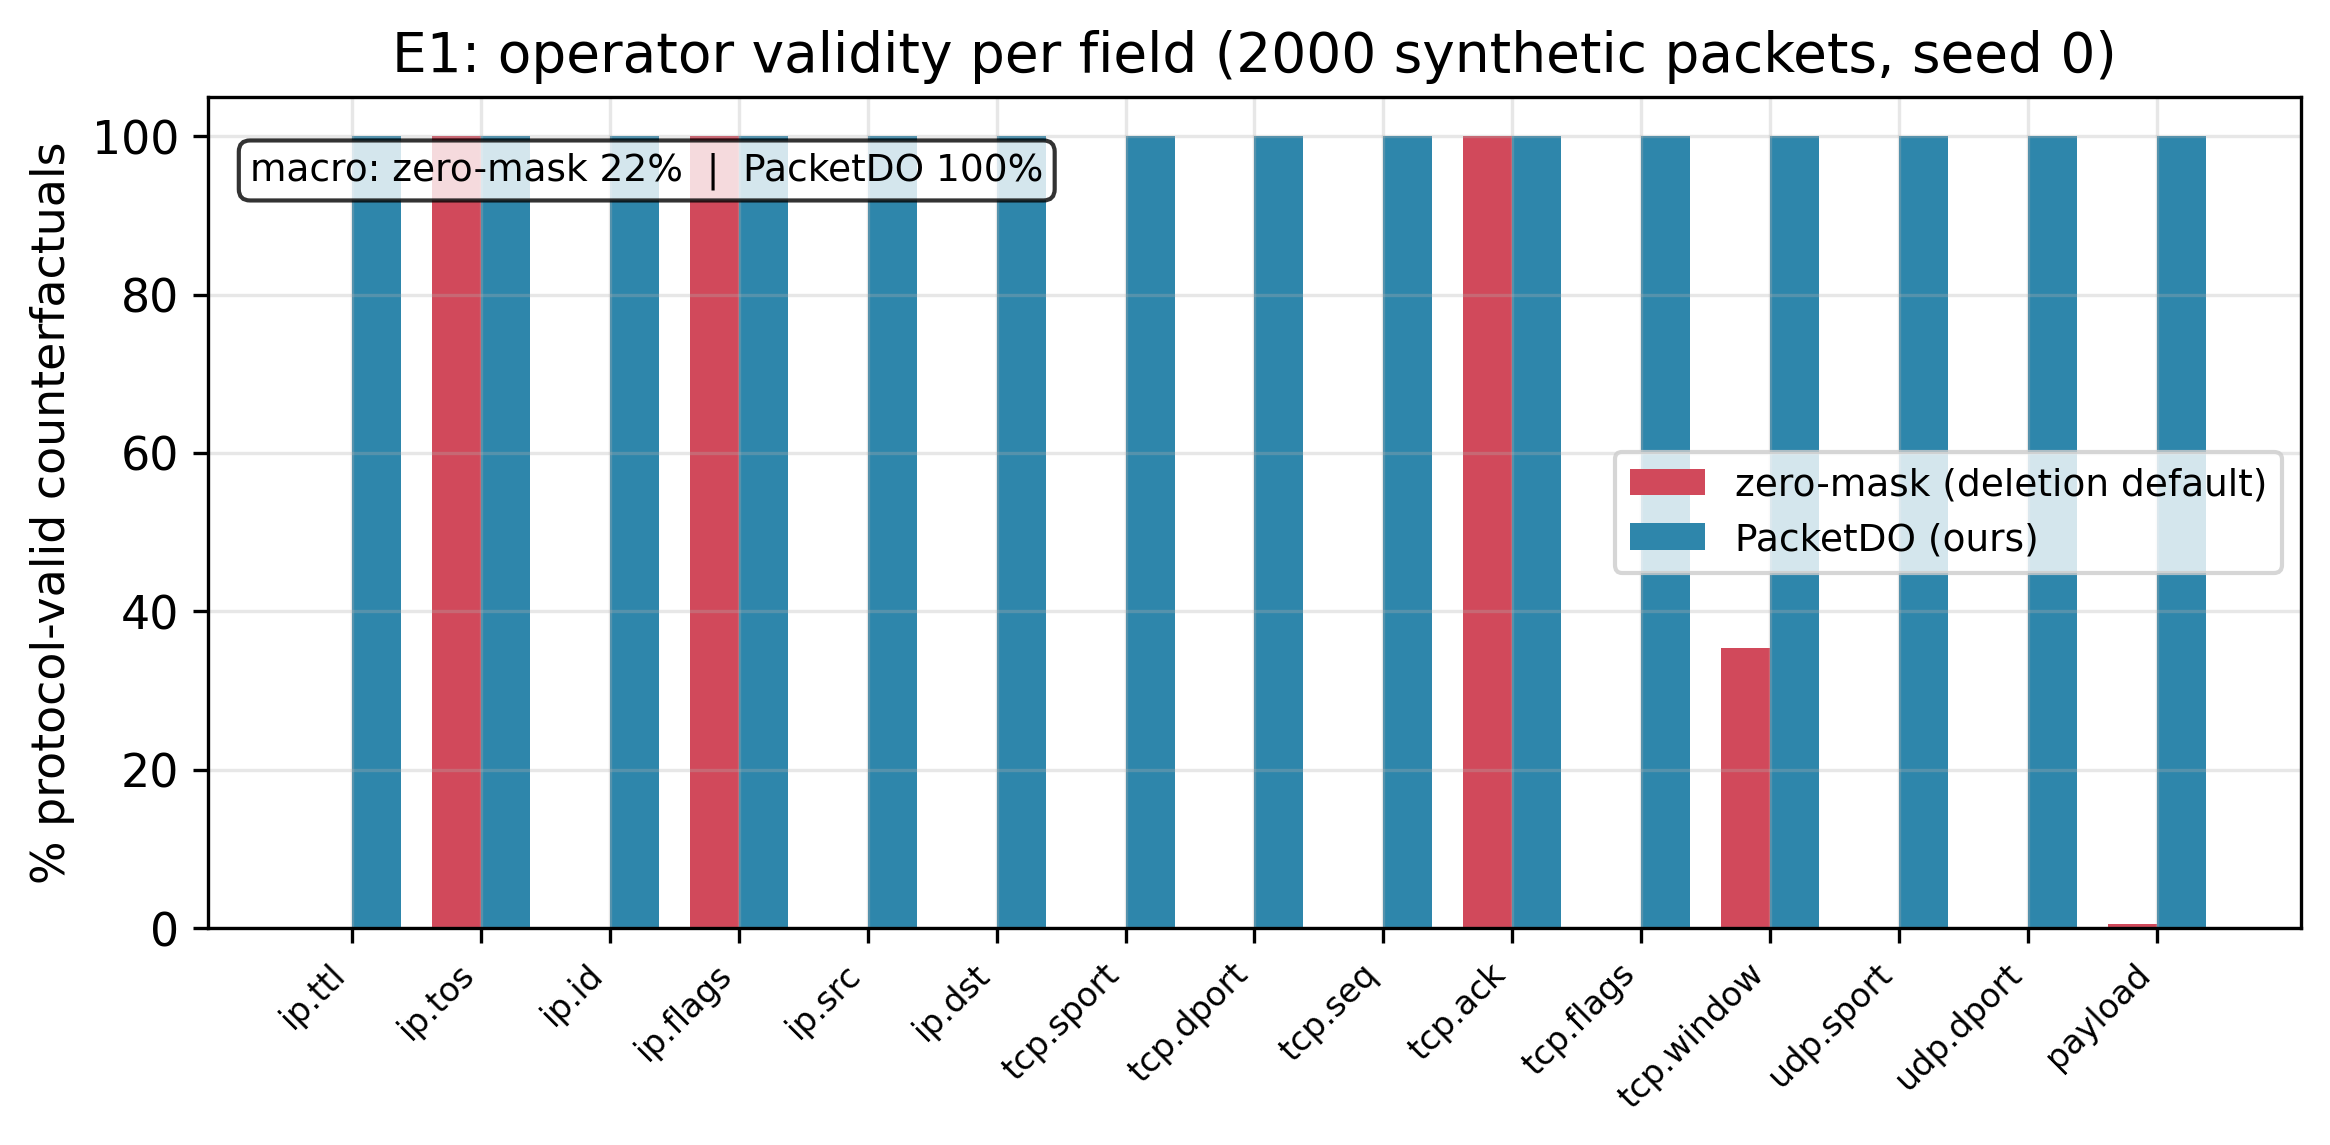
\includegraphics[width=\columnwidth]{figures/fig1_operator_validity.png}
\caption{Per-field protocol-validity of counterfactuals under zero-masking vs.\ PacketDO. Zero-masking is valid only where it is a no-op; PacketDO is valid by construction.}
\label{fig:validity}
\end{figure}

\subsection{E2, E3, E6: model fit, reliance on the planted artifacts,
and a clean null control}

Both models fit the planted task and improve with planting strength
(E2): ByteCNN test accuracy rises from 0.769 $\pm$ 0.007 at p=0.5 to 0.994 $\pm$
0.005 at p=1.0, and the RandomForest from 0.834 $\pm$ 0.006 to 1.000 $\pm$
0.000, so necessity is measured on competent models. The ByteCNN's
interventional necessity for the planted tcp.window shortcut rises from
0.273 $\pm$ 0.011 at planting strength p=0.5 to 0.501 $\pm$ 0.020 at p=1.0,
while its necessity for the equally-predictive ip.ttl shortcut stays at
or below 0.004: given two perfectly-correlated shortcuts the model
commits to one and ignores the other, so its redundancy degree $R(M)$=1
even though the data offers two. The null-intervention control
(tcp.sport, never correlated with the label) has a per-strength mean
necessity within $\pm$0.004 of zero across all cells (individual seeds range
up to $\pm$0.015), calibrating the estimator's noise floor.

\begin{figure}[!t]
\centering

\includegraphics[width=\columnwidth]{figures/fig3_necessity.png}
\caption{Interventional necessity $N(F)$. Models commit to \texttt{tcp.window} and ignore the redundant \texttt{ip.ttl}; the null field \texttt{tcp.sport} stays at zero.}
\label{fig:necessity}
\end{figure}

\textbf{R(M) validation.} To confirm the corrected estimator actually
measures redundancy, we validate it on oracle models with known
structure (Table II). An oracle that reads only tcp.window and one that
reads only ip.ttl each yield $R(M)$=1. A redundant oracle that trusts the
two markers when they agree and falls back to the genuine payload-length
signal when a resampled marker makes them disagree yields $R(M)$=2: each
shortcut alone recovers just under half the model's above-chance skill
under resampling, so the estimator returns two disjoint sufficient sets
for a sufficiency fraction up to 0.4 and a single joint set \{ip.ttl,
tcp.window\} at the stricter default 0.5. The removal-based
redundancy\_legacy returns R=1 for all three oracles, including the
redundant one, confirming that it cannot exceed one. The trained ByteCNN
and RandomForest at p=1.0 both commit to the single sufficient set
\{tcp.window\} ($R(M)$=1); their redundancy is therefore not within a run
but across training runs, and surfaces as the bimodal TreeSHAP false
confidence of Section 5.3. On real traffic the corrected estimator does
find within-model redundancy: a malware-family ByteCNN holds two
disjoint sufficient sets and the pretrained ET-BERT holds three ($R(M)$=2
and $R(M)$=3, Section 5.5), so R\textgreater1 is not confined to the
constructed oracle.

\begin{table}[!t]
\centering
\caption{$R(M)$ validation: removal-based (legacy) vs.\ sufficiency-based (corrected) redundancy on models with known structure ($p{=}1.0$); columns give the redundancy degree $R$. The legacy estimator cannot exceed~1; the corrected one recovers the intended $R{=}2$ for a redundant model.}
\label{tab:rm}
\small
\setlength{\tabcolsep}{4pt}
\begin{tabular}{@{}p{2.35cm}ccp{2.15cm}@{}}
\toprule
Model & Intended & Legacy & Corrected \\
\midrule
oracle: \texttt{tcp.window} only & 1 & 1 & 1 \\
oracle: \texttt{ip.ttl} only & 1 & 1 & 1 \\
oracle: window OR ttl (redundant) & 2 & 1 & 2 ($f{\leq}0.4$); 1 joint ($f{=}0.5$) \\
trained ByteCNN & n/a & 1 & 1 \\
trained RandomForest & n/a & 1 & 1 \\
\bottomrule
\end{tabular}
\end{table}

\subsection{E4: explainers find the shortcut but fabricate importance}

Every explainer ranks the model's true shortcut at the top (top-k
precision under the number-of-necessary-features convention is 1.0), so
the failure is not a missed truth. It is added falsehood, and it is
method- and strength-dependent:

\begin{itemize}
\tightlist
\item
  \textbf{Gradient saliency fabricates importance robustly:} CNN
  Saliency false-confidence is 0.684 $\pm$ 0.037 at p=1.0 and 0.68--0.74
  across all strengths, nonzero in all five seeds.
\item
  \textbf{Integrated Gradients and DeepSHAP fabricate importance
  conditionally:} IG false-confidence at p=1.0 is 0.300 $\pm$ 0.274 (nonzero
  in three of five seeds), the appealing seed-0 result of a clean
  endpoint does not generalize; DeepSHAP is clean at p$\geq$0.7 in all seeds
  but reaches 0.233 $\pm$ 0.325 at p=0.5 (fails in two of five seeds).
\item
  \textbf{Occlusion has zero false-confidence in every seed and
  strength}, but this is partly by construction: occlusion removes a
  feature by permutation, structurally close to the PacketDO
  ground-truth operator, so its clean record is not independent evidence
  and is disentangled in E5.
\item
  \textbf{Exactness does not confer faithfulness:} RF TreeSHAP
  false-confidence at p=1.0 is 0.200 $\pm$ 0.274, bimodal across seeds
  ({[}0.5, 0.5, 0, 0, 0{]}); it is 0.5 precisely in the seeds where the
  forest commits to one of the two correlated shortcuts and 0 when it
  spreads reliance. Exact Shapley values split credit by the data's
  correlation structure, so whenever a model commits to one of several
  redundant shortcuts they fabricate confidence in the unused one.
\end{itemize}

\begin{table*}[!t]
\centering
\caption{Explainer false-confidence rate (mean $\pm$ sd over 5 seeds) vs.\ planting strength. This table covers six of the eight audited methods; the two perturbation-based explainers, KernelSHAP and LIME, are computed on a subset for cost and reported separately in Section~5.4.}
\label{tab:fc}
\small
\begin{tabular}{@{}llcccc@{}}
\toprule
Method & Model & $p{=}0.5$ & $p{=}0.7$ & $p{=}0.9$ & $p{=}1.0$ \\
\midrule
Saliency & ByteCNN & $0.74\pm0.05$ & $0.70\pm0.05$ & $0.72\pm0.05$ & $0.68\pm0.04$ \\
IntegratedGradients & ByteCNN & $0.70\pm0.05$ & $0.57\pm0.09$ & $0.40\pm0.22$ & $0.30\pm0.27$ \\
DeepSHAP & ByteCNN & $0.23\pm0.33$ & $0.00\pm0.00$ & $0.00\pm0.00$ & $0.00\pm0.00$ \\
Occlusion & ByteCNN & $0.00\pm0.00$ & $0.00\pm0.00$ & $0.00\pm0.00$ & $0.00\pm0.00$ \\
Impurity & RF & $0.63\pm0.00$ & $0.00\pm0.00$ & $0.13\pm0.18$ & $0.20\pm0.27$ \\
TreeSHAP & RF & $0.00\pm0.00$ & $0.00\pm0.00$ & $0.33\pm0.00$ & $0.20\pm0.27$ \\
\bottomrule
\end{tabular}
\end{table*}

\begin{figure}[!t]
\centering
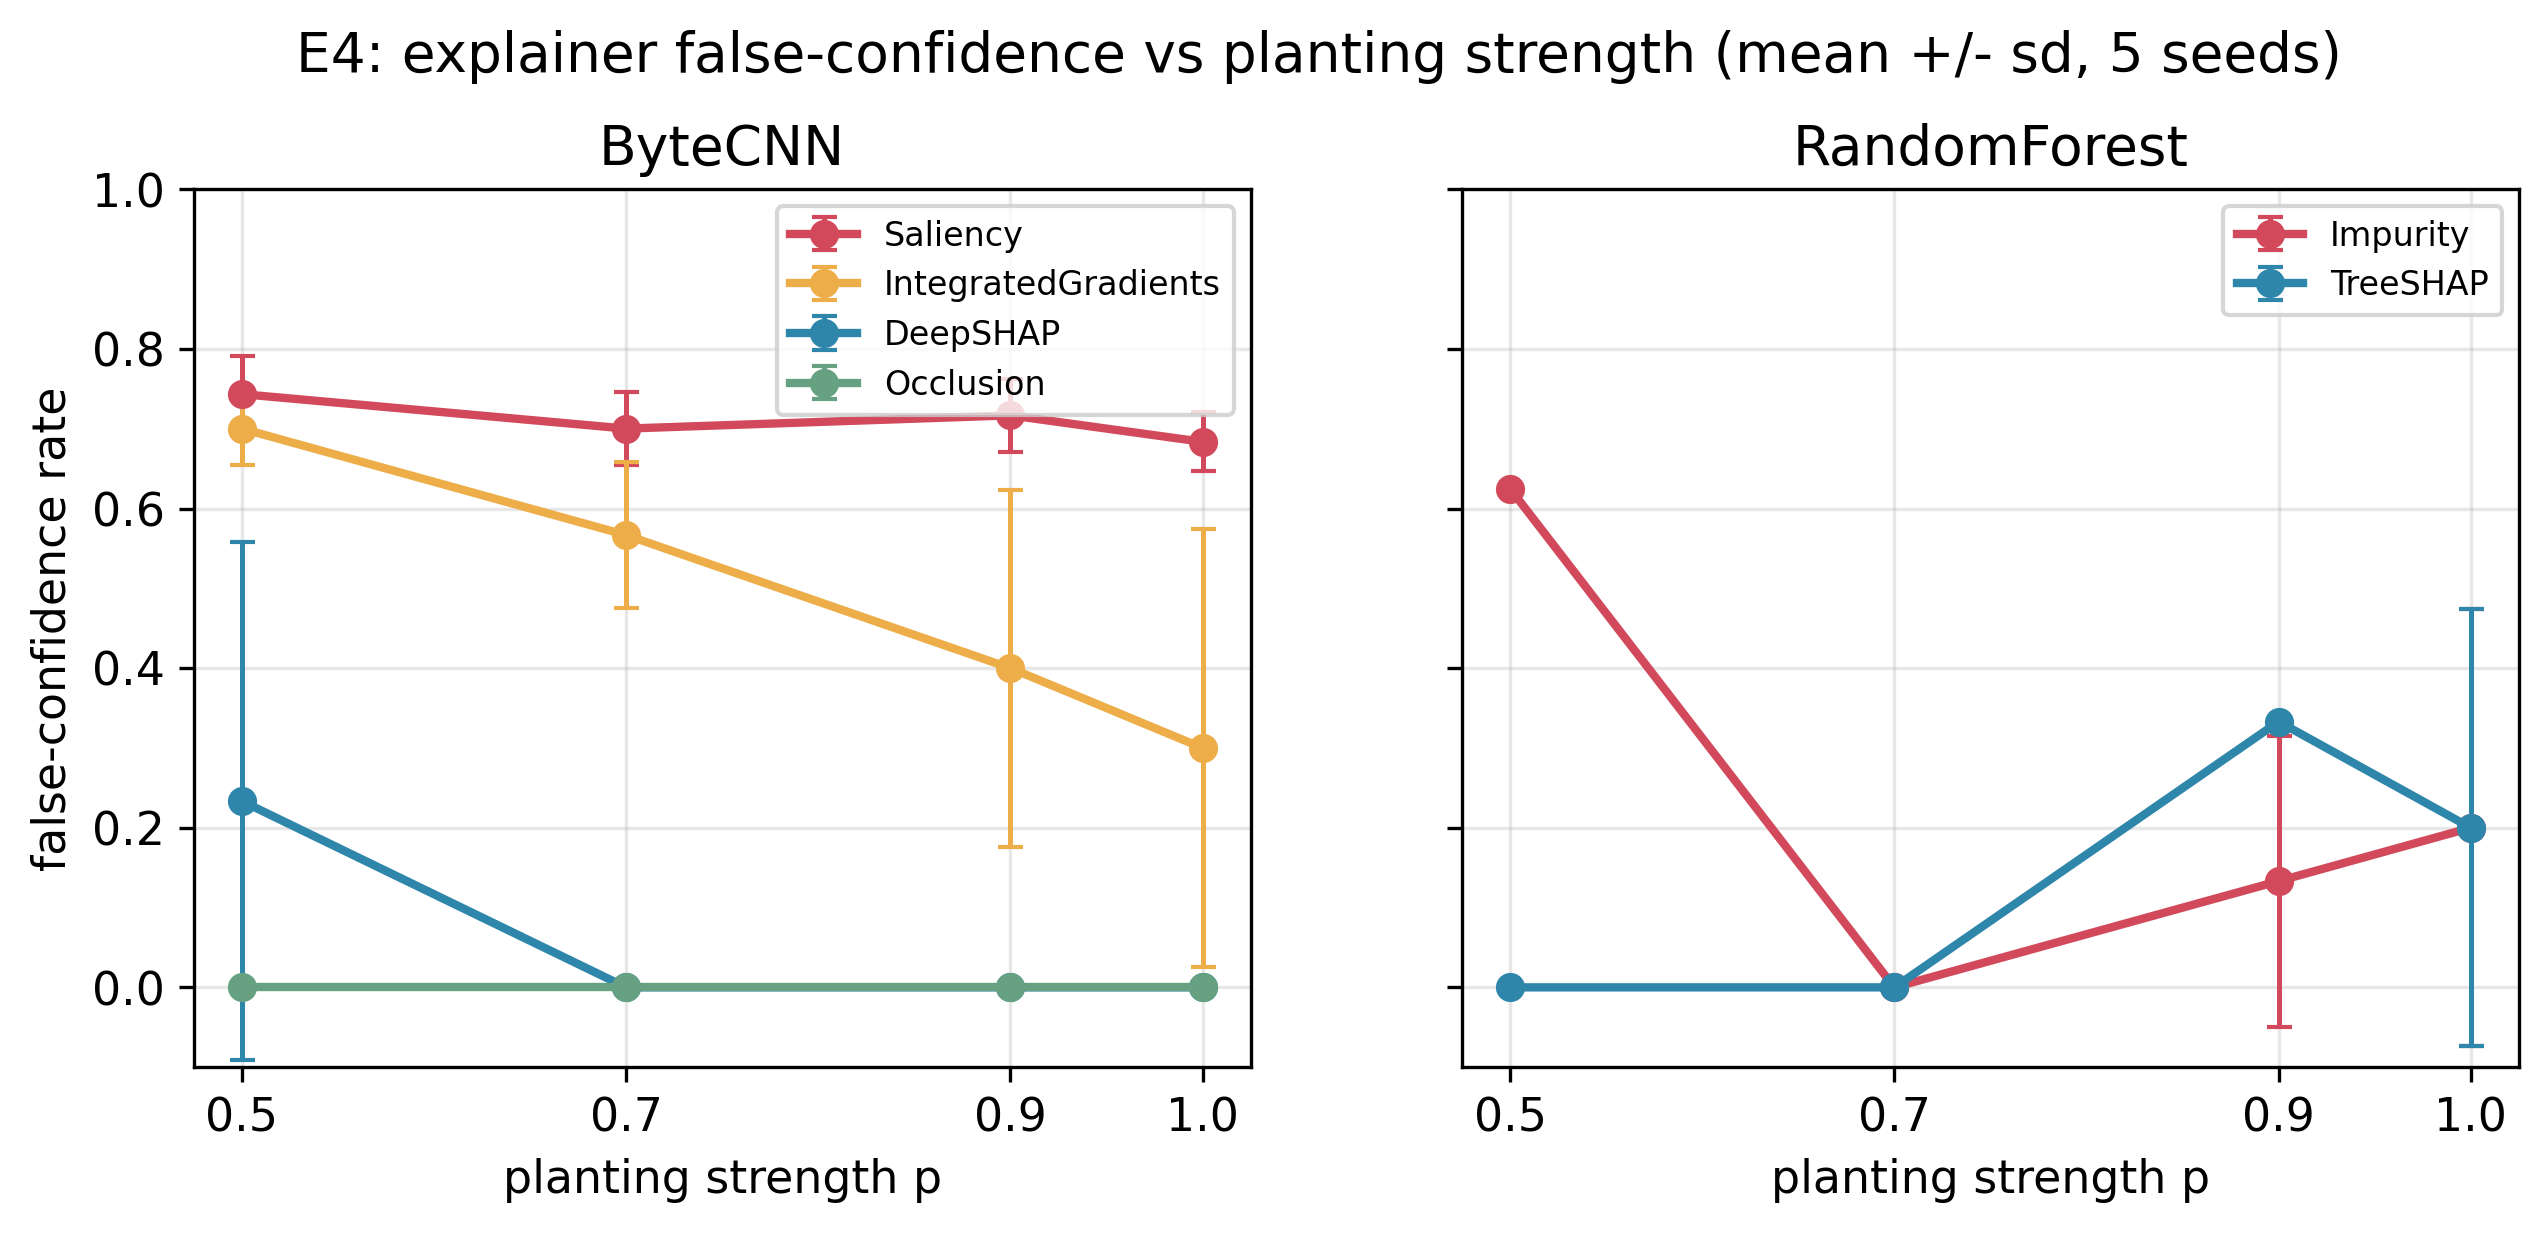
\includegraphics[width=\columnwidth]{figures/fig2_false_confidence.png}
\caption{False-confidence rate (fraction of confidently-attributed fields with interventional necessity ${\sim}0$) vs.\ planting strength, mean $\pm$ sd over 5 seeds. Gradient saliency fabricates importance robustly (0.68--0.74); Integrated Gradients and DeepSHAP do so conditionally (nonzero in 3/5 and 2/5 seeds respectively at their worst strength); occlusion is clean (partly by construction, see E5); RF TreeSHAP is bimodal, fabricating confidence exactly when the model commits to one of two redundant shortcuts.}
\label{fig:fc}
\end{figure}

\textbf{Real data.} On real CIC-IDS2017 flow data the same phenomena
appear on a documented natural artifact, and they survive a robustness
sweep over four RNG seeds and an alternative forest configuration (six
full-pipeline runs). A random forest (seed-0 test accuracy 0.99789,
macro-F1 0.91494) depends on the destination-port shortcut more than on
any other feature: its interventional necessity is 0.00434 $\pm$ 0.00012 in
accuracy (rank 1 of 52) and 0.04792 $\pm$ 0.00134 in macro-F1 at seed 0, and
destination port is the rank-1 accuracy-necessity feature of all 52 in
\emph{every} one of the six robustness runs (cross-run magnitude 0.00405
$\pm$ 0.00140; the $\pm$ on the seed-0 value is permutation-repeat noise, not
seed variance). Intervening on it collapses Brute-Force recall by 37.8
points (0.980 $\rightarrow$ 0.602) at seed 0 while leaving the port-spread
Port-Scanning class unaffected; Brute Force is the largest per-class
recall drop in every robustness run, at -35.3 $\pm$ 8.1 points across the
six (range -20.0 to -44.1).

Yet global TreeSHAP ranks destination port only 5th of 52 at seed 0, and
never better than 5th in any robustness run (rank 5--9 across the six,
mean 6.67 $\pm$ 1.63; Gini impurity buries it at 13--21). Nine of TreeSHAP's
top ten features at seed 0 are length statistics whose individual
accuracy-necessity is below 0.002, false confidence under the
accuracy-only criterion (eight of the nine belong to the packet-length
family used for the group-necessity probe below), and at least eight of
ten are false-confident in every robustness run (8.83 $\pm$ 0.41). These
same features have small but nonzero F1-necessity, so under a joint
accuracy-and-F1 criterion the false-confidence set shrinks to empty or a
single feature (0--1 of 10 across the six runs). Sweeping the necessity
cutoff makes this precise (Fig 4): the accuracy-only false-confidence
count is robust, holding at 8 to 10 of the top ten as the cutoff ranges
over two orders of magnitude (0.0005 to 0.05), so it is not an artifact
of the 0.002 threshold; additionally requiring low F1-necessity drops
the count to zero, because these length features carry minority-class F1
signal (F1-necessity 0.005 to 0.05) while moving overall accuracy by
less than 0.002. The false confidence is therefore genuine under an
accuracy criterion and criterion-dependent under an F1 one. The honest
headline is the redundancy mechanism: the packet-length family has group
necessity 0.201 in accuracy / 0.609 in F1 versus at most 0.00064
individually (seed 0), so credit-splitting floods the top of the global
ranking; the family fills 7--8 of the top-10 SHAP slots in every run.
The one robustness run with 8/10 rather than 9/10 is itself the
synthetic benchmark's model-commitment phenomenon on real data: at that
seed the forest makes one member of the redundant family genuinely
necessary, and exactly that feature exits the false-confidence set. The
single most F1-necessary feature (Fwd IAT Min) is TreeSHAP rank 36 of
52, a blind spot (seed-0 ranking; its position in the top three
accuracy-necessity features recurs in all six runs, but per-run SHAP
ranks below the top ten were not retained). The Engelen TCP-appendix
flow-construction artifact \cite{engelen2021troubleshooting} is present
as expected: its signature (Init\_Win\_bytes\_forward = -1 on benign
flows) appears on the original dataset and vanishes on the corrected
one.

\begin{figure*}[!t]
\centering
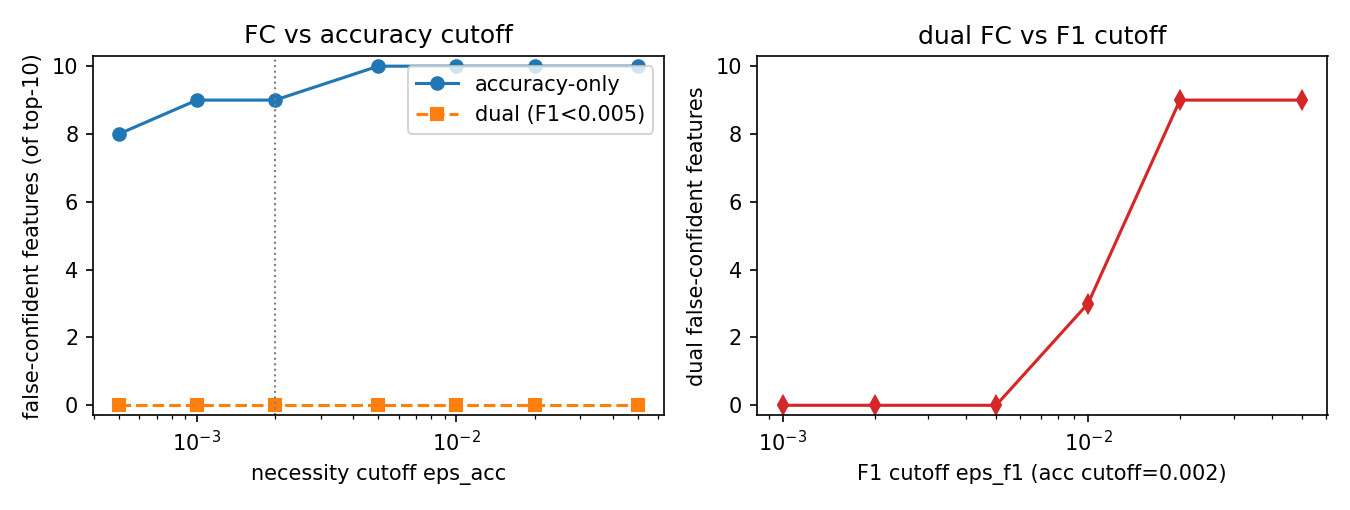
\includegraphics[width=0.92\textwidth]{figures/fc_sensitivity.png}
\caption{Threshold sensitivity of the real-data false-confidence count among TreeSHAP's top-10 features. Left: accuracy-only false confidence is flat at 8--10 as the necessity cutoff sweeps over two orders of magnitude, while the dual accuracy-and-F1 criterion (F1 cutoff 0.005) is zero throughout. Right: the dual count rises from 0 to 9 as the F1 cutoff is relaxed, showing the top features carry minority-class F1 signal even though their accuracy-necessity is near zero.}
\label{fig:fcsens}
\end{figure*}

\subsection{KernelSHAP, LIME, and cost}

Adding the two perturbation-based methods the audit lacked: KernelSHAP
has zero false-confidence but costs 10.8 s per 100 samples; LIME has
false-confidence 0.667 at 1.0 s per 100 samples, and the cause is
instructive: LIME's tabular perturbation standardizes features, and
scikit-learn's StandardScaler assigns unit scale to zero-variance
columns, so LIME perturbs constant protocol fields (a fixed destination
port, an address prefix) with unit-variance noise and reads the model's
response to those protocol-impossible inputs as importance. The
off-manifold problem this paper identifies reappears inside LIME's own
perturbation kernel.

\subsection{Byte-level replication on real packet captures}

To test the operator and the audit where the thesis actually applies, on
real packets rather than synthetic traffic or flow features, we run a
byte-level study on the ISCX VPN capture (facebook over TCP/443 vs ftps,
5,000 real packets per class, every packet carrying TCP options). A
ByteCNN reaches 0.979 test accuracy. Both load-bearing findings from the
synthetic benchmark reproduce on real bytes.

First, the operator gap is larger, not smaller, on real traffic
(E1-real). The captured packets are 100\% valid; zero-masking an
intervenable field leaves a protocol-valid packet in only 6.2\% of field
interventions (it breaks the IP checksum in 51,550 cases and the
transport checksum in 96,118), whereas PacketDO is valid in 100\% with
zero violations, including on the twelve TCP-option bytes per packet
that the synthetic population did not contain. The 6.2\% is below the
synthetic 22.4\% precisely because real packets carry options, giving
zero-masking more structure to break. This directly answers the concern
that PacketDO's validity might be a synthetic-serializer artifact: it
holds on real, option-laden, captured packets.

Second, the explainers again fabricate importance (Table IV).
Interventional necessity shows the model committed to the server
identity: N(ip.dst)=0.250 and N(ip.src)=0.163 dominate, every transport
and payload field is below 0.02, and the redundancy estimator returns a
single sufficient set \{ip.dst, ip.src\} ($R(M)$=1). Against this ground
truth the gradient explainers have false-confidence 0.71 (integrated
gradients) and 0.78 (saliency) and miss half the necessary fields
(precision@k and blind-spot both 0.5): on real packets they are worse
than on synthetic, confidently attributing importance to transport-layer
bytes the model provably does not use while overlooking one of the two
address fields it does. Occlusion is again the cleanest
(false-confidence 0.33, blind-spot 0), subject to the same
by-construction caveat (Section 8). The model's reliance on the server
address is itself the kind of shortcut the field warns about: it will
not transfer to the same applications on new hosts.

Third, the phenomenon transfers to an attention-based architecture,
though which explainer fails is model-dependent. We train a compact
byte-level Transformer encoder (two self-attention layers, four heads, a
CLS token, and learned positional embeddings) on the same task; it
reaches perfect test accuracy and, by intervention, commits to the same
server-identity shortcut (N(ip.src)=0.214, N(ip.dst)=0.195, every other
field at zero). On this model the gradient and occlusion explainers are
faithful (integrated gradients and occlusion both reach zero
false-confidence, occlusion rank correlation 0.975), where integrated
gradients had fabricated on the CNN; but attention-as-explanation is the
least faithful of the four (Table IV, Transformer block): reading the
CLS token's attention over the input bytes gives false-confidence 0.80
and blind-spot 0.5, attending confidently to fields the model provably
does not use while missing one of the two address fields it does. The
contested practice of treating attention weights as an explanation fails
here on exactly the architecture that motivates it, and in the direction
our audit is built to detect. This is a compact transformer trained from
scratch, not the pretrained ET-BERT whose fine-tuning pipeline we do not
reproduce; it is of the same architectural family, and it shows the
operator and the audit apply unchanged to self-attention.

We confirm this on the actual pretrained ET-BERT \cite{lin2022etbert}
rather than a from-scratch model. We load its released BERT-base weights
(verified against the original encoder to a maximum hidden-state
difference of 0.012), fine-tune on the same facebook-vs-ftps task to
perfect accuracy, and feed it the same 80-byte header window so the
comparison is apples-to-apples. The pretrained model commits to the
server identity as well (N(ip.dst)=0.068, N(ip.src)=0.055, every other
field zero), and here the redundancy is stronger still: the corrected
estimator returns $R(M)$=3, three disjoint sufficient sets \{ip.src\},
\{ip.dst\}, and \{tcp.sport, tcp.dport\}, so the attribution target is
maximally non-unique. All three explainers we run on it fabricate
importance against this ground truth (Table IV, ET-BERT block):
attention, saliency, and integrated gradients rank the address fields at
the top (precision@k 1.0) yet carry false-confidence 0.71, 0.80, and
0.60, attributing importance to fields the model provably does not use.
The false-confidence phenomenon therefore holds on the exact pretrained
transformer the field deploys, not only on our from-scratch model. (We
audit ET-BERT on the header window for comparability; its native
payload-burst tokenization is a separate input regime, noted in Section
9.)

Fourth, both findings hold on a second, unrelated corpus. We replicate
the byte-level study on USTC-TFC2016 \cite{wang2017malware} as a
malware-family task (Miuref vs Geodo, 5,000 real packets per class);
unlike the raw-IP ISCX subset these captures are Ethernet-framed and are
normalized to IP before the identical pipeline runs. The operator gap
holds and is again large: zero-masking is valid for only 15.5\% of field
interventions (breaking the IP checksum in 48,643 cases and the
transport checksum in 72,133) versus 100\% for PacketDO. The gradient
explainers again fabricate importance (integrated gradients and saliency
false-confidence 0.67 and 0.78 against a ByteCNN, test accuracy 0.864,
that commits to the destination address, N(ip.dst)=0.130, while
confidently ranking the unused IP TTL, N=0.026, near the top), and
occlusion is again clean. Here the model holds two substitutable
shortcuts and the corrected redundancy estimator returns $R(M)$=2 with
disjoint sufficient sets \{ip.dst\} and \{tcp.window\}: this is the
redundancy of Section 5.2 found in a trained model on real traffic
rather than a constructed oracle, and it makes the attribution target
genuinely non-unique.

\begin{table*}[!t]
\centering
\caption{Real byte-level audit across two capture corpora (ISCX VPN facebook/ftps; USTC-TFC2016 Miuref/Geodo), single run per corpus. Models: ByteCNN (ISCX accuracy 0.979, USTC 0.864) and, on ISCX, a compact self-attention Transformer and the pretrained ET-BERT (BERT-base), both at accuracy 1.0. Necessity is measured by PacketDO on the real packets; false-confidence and blind-spot are computed against it.}
\label{tab:realbyte}
\small
\begin{tabular}{@{}llcccc@{}}
\toprule
Corpus / model & Method & $\rho$ & precision@$k$ & False-confidence & Blind-spot \\
\midrule
ISCX / ByteCNN & IntegratedGradients & 0.389 & 0.50 & 0.714 & 0.50 \\
ISCX / ByteCNN & Saliency & 0.195 & 0.50 & 0.778 & 0.50 \\
ISCX / ByteCNN & Occlusion & 0.485 & 1.00 & 0.333 & 0.00 \\
\addlinespace
ISCX / Transformer & IntegratedGradients & 0.683 & 1.00 & 0.000 & 0.00 \\
ISCX / Transformer & Saliency & 0.701 & 1.00 & 0.333 & 0.00 \\
ISCX / Transformer & Occlusion & 0.975 & 1.00 & 0.000 & 0.00 \\
ISCX / Transformer & Attention & 0.588 & 0.50 & 0.800 & 0.50 \\
\addlinespace
ISCX / ET-BERT (pretrained) & Attention & 0.701 & 1.00 & 0.714 & 0.00 \\
ISCX / ET-BERT (pretrained) & Saliency & 0.701 & 1.00 & 0.800 & 0.00 \\
ISCX / ET-BERT (pretrained) & IntegratedGradients & 0.683 & 1.00 & 0.600 & 0.00 \\
\addlinespace
USTC / ByteCNN & IntegratedGradients & 0.734 & 0.50 & 0.667 & 0.50 \\
USTC / ByteCNN & Saliency & 0.471 & 0.50 & 0.778 & 0.50 \\
USTC / ByteCNN & Occlusion & 0.423 & 1.00 & 0.000 & 0.00 \\
\bottomrule
\end{tabular}
\end{table*}

\section{E5: faithfulness verdicts depend on the removal operator}

For the p=1.0 ByteCNN, we score each explainer with a standard
deletion-AOPC curve under two removal operators. Under zero-masking the
four methods order IG (0.4776) \textgreater{} Saliency (0.4730)
\textgreater{} DeepSHAP (0.4724) \textgreater{} Occlusion (0.4629), a
spread of 0.0147; under PacketDO they collapse to within 0.0010, below
the per-seed resampling noise (\textasciitilde0.0058). The Kendall tau
between the two orderings is 0.333. The robust and load-bearing effect
is not the full four-way reordering (the middle ranks differ by less
than one test-sample count) but a specific demotion: under zero-masking,
occlusion, the method with zero false-confidence and the best
necessity-rank correlation (0.715), is ranked last, below saliency,
whose false-confidence is 0.667 and whose necessity correlation is
0.043. The protocol- invalid operator manufactures an ordering that
inverts the audit evidence, and it does so on non-monotone deletion
curves computed on impossible packets. Any comparison of
traffic-classifier explainers that used the zero-masking operator, the
field default, therefore inherits an ordering that is an artifact of the
operator, not a property of the explanations (contribution C4).

\begin{table}[!t]
\centering
\caption{E5: deletion AOPC of each explainer under zero-mask vs.\ PacketDO removal ($p{=}1.0$ ByteCNN; PacketDO mean over 5 resampling seeds). Higher AOPC $=$ steeper deletion $=$ nominally more faithful. Under zero-mask, Occlusion (false-confidence~0) is ranked last; under PacketDO the four are within 0.001 (below resampling noise ${\sim}0.006$).}
\label{tab:e5}
\small
\setlength{\tabcolsep}{4pt}
\begin{tabular}{@{}lccc@{}}
\toprule
Explainer & Zero-mask & PacketDO & FC \\
          & AOPC      & AOPC     & (seed 0) \\
\midrule
IntegratedGradients & 0.4776 & 0.4882 & 0.0 \\
Saliency & 0.4730 & 0.4875 & 0.667 \\
DeepSHAP & 0.4724 & 0.4872 & 0.0 \\
Occlusion & 0.4629 & 0.4881 & 0.0 \\
\bottomrule
\end{tabular}
\end{table}

\section{Discussion and implications}

\textbf{The failure is added falsehood, not missed truth.} Across every
model, dataset, and planting strength, the explainers we tested rank a
model's genuinely-used feature at or near the top: on the synthetic
benchmark precision-at-k is 1.0, and on real CIC-IDS2017 the
destination-port shortcut that the model most depends on is surfaced by
per-class SHAP. What the explainers add is confident, high-magnitude
importance for features the model provably does not use. On the
synthetic benchmark this shows up as gradient-saliency false-confidence
around 0.7; on real data it is starker, because the redundant features
are numerous: nine of TreeSHAP's global top ten are length statistics
that are collectively load-bearing but individually near-zero in
interventional necessity, and they outrank the single most necessary
feature. An operator reading the explanation cannot separate the feature
the model uses from the many it merely could have used. This is a more
dangerous failure than a low-quality but honest ranking, because the
false positives are exactly the plausible-looking features that invite a
wrong intervention.

\textbf{Redundancy makes single-explanation evaluation ill-posed, and
exactness does not help.} The reason the false positives appear is
structural: traffic data encodes the same discriminative signal many
times over (two headers that both leak the class, a family of correlated
flow statistics) so a model is free to commit to one encoding and ignore
the rest, and different models (or the same architecture under a
different seed) commit differently. An attribution method that returns a
single importance vector is answering a question with no unique answer.
TreeSHAP makes this precise: it computes exact Shapley values, and it
still fabricates confidence in an unused shortcut, because Shapley
values distribute credit according to the correlation structure of the
data rather than the realized reliance of the model. Exactness of the
attribution is orthogonal to its faithfulness when the explanandum is
not unique. Our redundancy degree $R(M)$ is the property that has to be
measured before a single-vector explanation can even be interpreted, and
it is measurable only by intervention.

\textbf{The removal operator is not a detail.} E5 shows that the ranking
of explainers by a standard deletion-style faithfulness score can invert
depending on whether features are removed by zero-masking or by
PacketDO: under the protocol-invalid zero-mask operator the method with
zero false-confidence (occlusion) is ranked worst, below a method with
high false-confidence, because the zero-masked inputs are off-manifold
and the resulting deletion curves are not even monotone. Under the
protocol-valid operator the methods that all correctly identify the
model's single true shortcut collapse, correctly, to a spread below the
resampling noise. Any comparison of explainers for traffic classifiers
that used the zero-masking operator, the field default, therefore
inherits an ordering that is an artifact of the operator, not a property
of the explanations. The same off-manifold mechanism reappears inside an
explainer: LIME's false-confidence traces to its perturbation kernel
sampling constant protocol fields with unit variance (an artifact of
standardizing zero-variance features), i.e.~LIME evaluates the model on
impossible packets as part of its own definition.

\textbf{Why this matters operationally.} The traffic-classification
literature does not stop at displaying attributions. Deployed and
published systems act on them: xNIDS \cite{wei2023xnids} generates
active intrusion-response rules from its explanations, ShortcutCatcher
\cite{zhao2026shortcutcatcher} deletes features from the training
pipeline based on what an explainer flags, and analyst-facing tools
present attributed features as the justification for an alert. A
false-confidence feature in that setting is not a mislabeled figure; it
is a firewall rule keyed on a coincidence, a genuinely-predictive
feature wrongly pruned, or an analyst's trust spent on the wrong
evidence. The interventional reference we provide is the check these
pipelines currently lack: before an attribution is allowed to drive an
action, it can be scored against what the model actually depends on.

\textbf{What we do not claim.} We do not claim explanations are
worthless, nor that any single method is uniformly best.
Intervention-aligned methods (occlusion, and DeepSHAP at sufficient
signal strength) are the most faithful in our study, but occlusion's
advantage is partly structural: it removes features much as our
ground-truth operator does, so its clean record is not independent
evidence (Section 8), and even it is only as good as the removal
operator it uses; DeepSHAP fails at weak planting strength in a subset
of seeds. The constructive reading of our results is that faithfulness
for traffic classifiers is achievable, but only with a protocol-valid
intervention and an explicit accounting of redundancy; neither is
present in current practice.

\section{Threats to validity}

\textbf{Resampling changes the joint distribution.} PacketDO preserves
each field's marginal but, by sampling it independently of the label,
alters its joint distribution with the other fields. A model that relied
on a genuine correlation between two fields would register a necessity
drop that is real but not attributable to either field alone. We
mitigate this in three ways: interventions resample class-agnostically
from real values (so every counterfactual is a value the field actually
takes); we report field-set necessity for the documented redundant
families, not only single-field necessity; and we include a
null-intervention control field in every table, whose necessity stays
within the noise floor and calibrates what ``zero necessity'' means for
the estimator.

\textbf{The model must not be retrained under intervention.} Necessity
and sufficiency are properties of a fixed model; retraining after an
intervention (as remove-and-retrain protocols do
\cite{hooker2019benchmark}) measures a different model and reintroduces
the confound our operator was designed to avoid. We freeze the model for
all interventions. Where a strength sweep requires different models,
each strength is trained once before any intervention is applied to it.

\textbf{Byte-versus-field granularity.} Byte-level explainers attribute
to byte offsets, which we aggregate to protocol fields using a fixed
header-offset map valid for the canonical no-options layout. Two
consequences: attributions to bytes shared by two fields, or to
variable-length options, are aggregated approximately; and where header
lengths differ across samples (the misalignment that motivates
protocol-aware parsing) absolute offsets are not stable. We report
results at both byte and field granularity and use protocol-parsed
offsets for the misaligned cases.

\textbf{Cost of exact methods.} KernelSHAP is orders of magnitude slower
than the gradient and tree methods; we bound it with stratified
subsampling and report the measured wall-clock cost, which is itself a
datapoint for line-rate deployment. This means KernelSHAP results are
computed on fewer samples than the other methods, with correspondingly
wider uncertainty.

\textbf{Occlusion is close to the ground-truth operator.} Occlusion
removes a feature by permutation, structurally similar to PacketDO's
resampling. Its strong faithfulness is therefore partly by construction,
and we state this explicitly rather than presenting occlusion as an
independent winner. E5 disentangles the effect by scoring occlusion
under both the zero-mask and PacketDO operators.

\textbf{The off-manifold claim is distributional, not absolute.} Our
argument is that a zero-masked packet lies off the distribution of
conforming traffic a classifier is trained on, not that such a packet
can never be observed. Malformed packets do occur, from NIC
checksum-offload capture, truncation, or adversarial crafting, and an
intrusion detector may even be required to classify them. The point is
narrower: attributions computed by deleting a field query the model on
inputs its training distribution does not contain, so the resulting
importance is confounded with extrapolation. PacketDO removes that
confound by keeping every counterfactual within the conforming-traffic
manifold; auditing robustness to genuinely malformed inputs is a
separate question we do not address here.

\textbf{Synthetic versus real.} The graded-strength results are on
synthetic traffic, where ground truth is planted and exact. Their
external validity rests on two real-data replications: a flow-level one
(CIC-IDS2017, Section 5.3), where the false-confidence and blind-spot
phenomena reproduce on documented natural artifacts, and byte-level ones
on two real packet-capture corpora (ISCX VPN app traffic and
USTC-TFC2016 malware traffic, Section 5.5), where the operator gap
(zero-mask 6.2\% vs PacketDO 100\% on option-laden real packets) and the
explainer false-confidence (0.71-0.78 for gradient methods) both
reproduce and are in fact stronger than on synthetic traffic. This
addresses the concern that PacketDO's validity or the audit result might
be artifacts of the synthetic generator. What we do not yet cover is the
full catalogue of documented byte-level artifacts (the ISCX
Ethernet-misalignment quirk, CIC-IDS-2017 TTL 64/128, sequence-number
bytes) as planted, graded ground truth; the ISCX captures we use are
raw-IP framed, so the misalignment artifact in particular is
dataset-specific and left to future work.

\begin{table*}[!t]
\centering
\caption{Real-data (CIC-IDS2017) destination-port robustness: 4 seeds $\times$ default RF (d20/l20) $+$ 2 alt-config runs (d30/l5). Necessity rank 1/52 in all six runs; TreeSHAP never ranks it better than 5th.}
\label{tab:robust}
\small
\begin{tabular}{@{}lcccc@{}}
\toprule
Run & $N(\mathrm{dst})$ acc-rank /52 & TreeSHAP rank /52 & Acc-only FC /10 & Brute-Force recall drop \\
\midrule
\texttt{default\_seed0} & 1 & 5 & 9 & 0.378 \\
\texttt{default\_seed1} & 1 & 7 & 8 & 0.441 \\
\texttt{default\_seed2} & 1 & 8 & 9 & 0.382 \\
\texttt{default\_seed3} & 1 & 9 & 9 & 0.199 \\
\texttt{alt\_d30l5\_seed0} & 1 & 5 & 9 & 0.360 \\
\texttt{alt\_d30l5\_seed1} & 1 & 6 & 9 & 0.356 \\
\bottomrule
\end{tabular}
\end{table*}

\textbf{Serializer circularity.} Both PacketDO's validity and the
validity checker rely on the same protocol serializer. We harden this in
two ways: the checker was cross-validated against a from-scratch
one's-complement (RFC 1071) checksum implementation on adversarial
corruptions, and the operator's per-field correctness is covered by unit
tests; an independent validator (e.g.~tshark) is a further step. The E1
macro-validity figure is an unweighted average over synthetic fields,
not a per-packet real-traffic rate, and three fields are valid under
zero-masking only because the generator left them zero; on real traffic
the zero-mask validity would if anything be lower, so the reported gap
is conservative.

\textbf{Seed sensitivity of quantized metrics.} False-confidence is a
fraction over a small set of named fields and therefore takes quantized
values (0, 1/3, 1/2, \ldots); a small rescaling of attributions can move
it between levels. We report it as a mean with standard deviation over
five seeds and give the per-seed values, and we distinguish claims that
hold in every seed (saliency false-confidence, occlusion's clean record)
from those that are seed-contingent (the exact strength at which
Integrated Gradients or DeepSHAP first fabricates importance). On the
real-data side, the six-run sweep spans four seeds and two forest
configurations; the alternative (deeper) configuration strengthens
rather than weakens the findings, so the artifact reliance is not an
under-fitting effect of the default configuration.

\section{Limitations and future work}

Our scope is the faithfulness axis of explanation quality for traffic
classifiers, evaluated with a protocol-valid intervention. Several
adjacent problems, identified in our systematic gap analysis of the
literature (see the supplementary gap-analysis document accompanying the
artifact release), are deliberately out of scope and define the research
programme this instrument enables:

\begin{itemize}
\item
  \textbf{Metric meta-evaluation (diagnosticity).} With planted-truth
  models in hand, the field's existing faithfulness \emph{metrics}
  (deletion-AUC, descriptive accuracy, fidelity) can themselves be
  scored on whether they distinguish faithful from unfaithful
  explainers. E5 is a first datapoint (the zero-mask AOPC ranking
  inverts the audit evidence); a systematic diagnosticity study is the
  natural sequel to this paper.
\item
  \textbf{Drift-aware evaluation.} Traffic distributions drift, and an
  explanation that is faithful at training time may not remain so under
  deployment drift \cite{pendlebury2019tesseract}. No
  temporal-drift-aware explanation evaluation exists for traffic; our
  interventional reference is recomputable at any time slice and could
  anchor one.
\item
  \textbf{The plausibility axis and analyst studies.} We measure whether
  explanations reflect the model, not whether they help an analyst
  \cite{jacovi2020towards,alquliti2025evaluating}. A two-axis protocol
  that scores plausibility and faithfulness separately (and the
  analyst-grounded human evaluation the security setting ultimately
  requires) are open, and our ground-truth tables provide the
  faithfulness half of such a protocol.
\item
  \textbf{Adversarial robustness of explainers.} An adversary can
  manipulate explanations \cite{slack2020fooling}; whether
  protocol-valid perturbations can be crafted to mislead traffic-model
  explainers, and whether interventional auditing detects such
  manipulation, is unstudied.
\item
  \textbf{Full redundancy (Rashomon) enumeration.} Our $R(M)$ counts
  disjoint sufficient field sets by forward selection against a
  sufficiency threshold; a complete enumeration of the Rashomon set of
  equally-performing models and their explanation multiplicity, and of
  $R(M)$ across the model distribution rather than a single trained model,
  is a larger undertaking that our credit-splitting and commitment
  results motivate.
\item
  \textbf{ET-BERT's native tokenization and the full artifact
  catalogue.} The audit spans a byte-CNN, a random forest, a compact
  self-attention Transformer, and the pretrained ET-BERT
  \cite{lin2022etbert}, across synthetic traffic, real flow features,
  and two real packet-capture corpora
  (\cite{drapergil2016vpn,wang2017malware}). Two extensions remain.
  First, we audit ET-BERT on the header window for comparability; its
  native payload-burst tokenization is a different input regime that
  does not use our fixed header-offset map and would need a
  token-to-field map of its own, so a payload-tokenized audit is a
  genuine extension. Second, planting the full catalogue of documented
  byte-level artifacts (the ISCX Ethernet-misalignment quirk,
  CIC-IDS-2017 TTL 64/128) as graded ground truth, rather than measuring
  the artifacts a given capture happens to contain.
\end{itemize}

\section{Reproducibility}

Every number in this paper traces to a versioned result file produced by
a seeded script, and the full pipeline runs on commodity hardware (CPU
for all tree-model and intervention experiments; a consumer laptop GPU
suffices for the ByteCNN and the perturbation explainers). The artifact
release contains: the PacketDO operator with its per-field unit-test
suite (42 passed, 1 skipped) and the RFC 1071 cross-validated validity
checker; the synthetic generator and per-strength planted-shortcut
datasets (seeded); the benchmark driver that trains both model families,
computes interventional ground truth, runs all eight explainers, and
audits them; the E5 operator-sensitivity driver; and the CIC-IDS2017
real-data pipeline with its six-run robustness harness (approximately
200--220 s per run on CPU; 1,232 s for all six). Multi-seed aggregation
is performed by a script that validates the provenance of every per-seed
result file (internal seed and strength fields must match the filename;
mismatched files are excluded and the run exits nonzero), a guard added
after it caught a file-duplication fault in an early automated run, and
callers are required to check its exit code. The seed-0 real-data
reference run is reproduced float-identically by the robustness
harness's first run. All datasets are public (CIC-IDS2017 original and
Engelen-corrected \cite{engelen2021troubleshooting}); the synthetic
traffic is regenerated from a seed. One top-level make target reproduces
every table and figure from a clean checkout.

\bibliographystyle{IEEEtran}
\bibliography{refs}

\end{document}
